\chapter{Исследовательская часть}

В данной части представляются технические характеристики, постановка, проведение и результаты исследования.

\section{Технические характеристики}

Спецификации устройства, использованного для тестирования:
\begin{itemize}[label=--]
	\item оперативная память 16 ГБ;
	\item процессор Intel(R) Core(TM) i7-9750H с тактовой частотой 2.60 ГГц;
	\item 6 физических и 12 логических ядер;
	\item операционная система Windows 10 Домашняя 64-разрядная с версией 22H2.
\end{itemize}

Устройство было нагружено только встроенными приложениями и подключено в сеть электропитания. 

\section{Постановка исследования}

Целью исследования является определение зависимостей:
\begin{itemize}[label=--]
	\item значения фундаментальной цены от количества участников;
	\item значения фундаментальной цены от стоимости мероприятия.
\end{itemize}

По результатам исследованя должны быть составлены таблицы и построены графики зависимости.

\section{Определение зависимости значения фундаментальной цены от количества участников}

Для определения зависимости используется мероприятие, состоящее из 3-х дней с одинаковой стоимостью.

Характеристики мероприятия для определения зависимости значения фундаментальной цены от количества участников представлены в таблице~\ref{tbl:event-chars-1}.

\begin{table}[H]
	\centering
	\caption{Характеристики мероприятия для определения зависимости значения фундаментальной цены от количества участников}
	\label{tbl:event-chars-1}
	\begin{tabularx}{\textwidth}{|X|X|X|X|}
		\hline
		\textbf{Характеристика} & \textbf{1 день} & \textbf{2 день} & \textbf{3 день} \\
		\hline
		Стоимость & 10000 & 15000 & 5000 \\
		\hline
		Коэффициент & 2 & 3 & 1 \\
		\hline
	\end{tabularx}
\end{table}

Результаты определения зависимости значения фундаментальной цены от количества участников представлены в таблицах~\ref{tbl:short-dependence-1}~и~\ref{tbl:dependence-1}.

\begin{table}[H]
	\centering
	\caption{Результаты определения зависимости значения фундаментальной цены от количества участников}
	\label{tbl:short-dependence-1}
	\begin{tabularx}{\textwidth}{|X|X|}
		\hline
		\textbf{Количество участников} & \textbf{Фундаментальная цена} \\
		\hline
		500  & 10.0000         \\ \hline
		450  & 11.1111         \\ \hline
		400  & 12.5000         \\ \hline
		350  & 14.2857         \\ \hline
		300  & 16.6667         \\ \hline
		250  & 20.0000         \\ \hline
		200  & 25.0000         \\ \hline
		150  & 33.3333         \\ \hline
		100  & 50.0000         \\ \hline
		50   & 100.0000        \\ \hline
		10   & 500.0000        \\ \hline
	\end{tabularx}
\end{table}

По таблице~\ref{tbl:dependence-1} был построен график~\ref{fig:dependency-1}, который наглядно демонстрирует результаты определения зависимости значения фундаментальной цены от количества участников. Исходя из графика можно сделать вывод, что данная зависимость близка к обратной.

\begin{figure}[H]
	\centering
	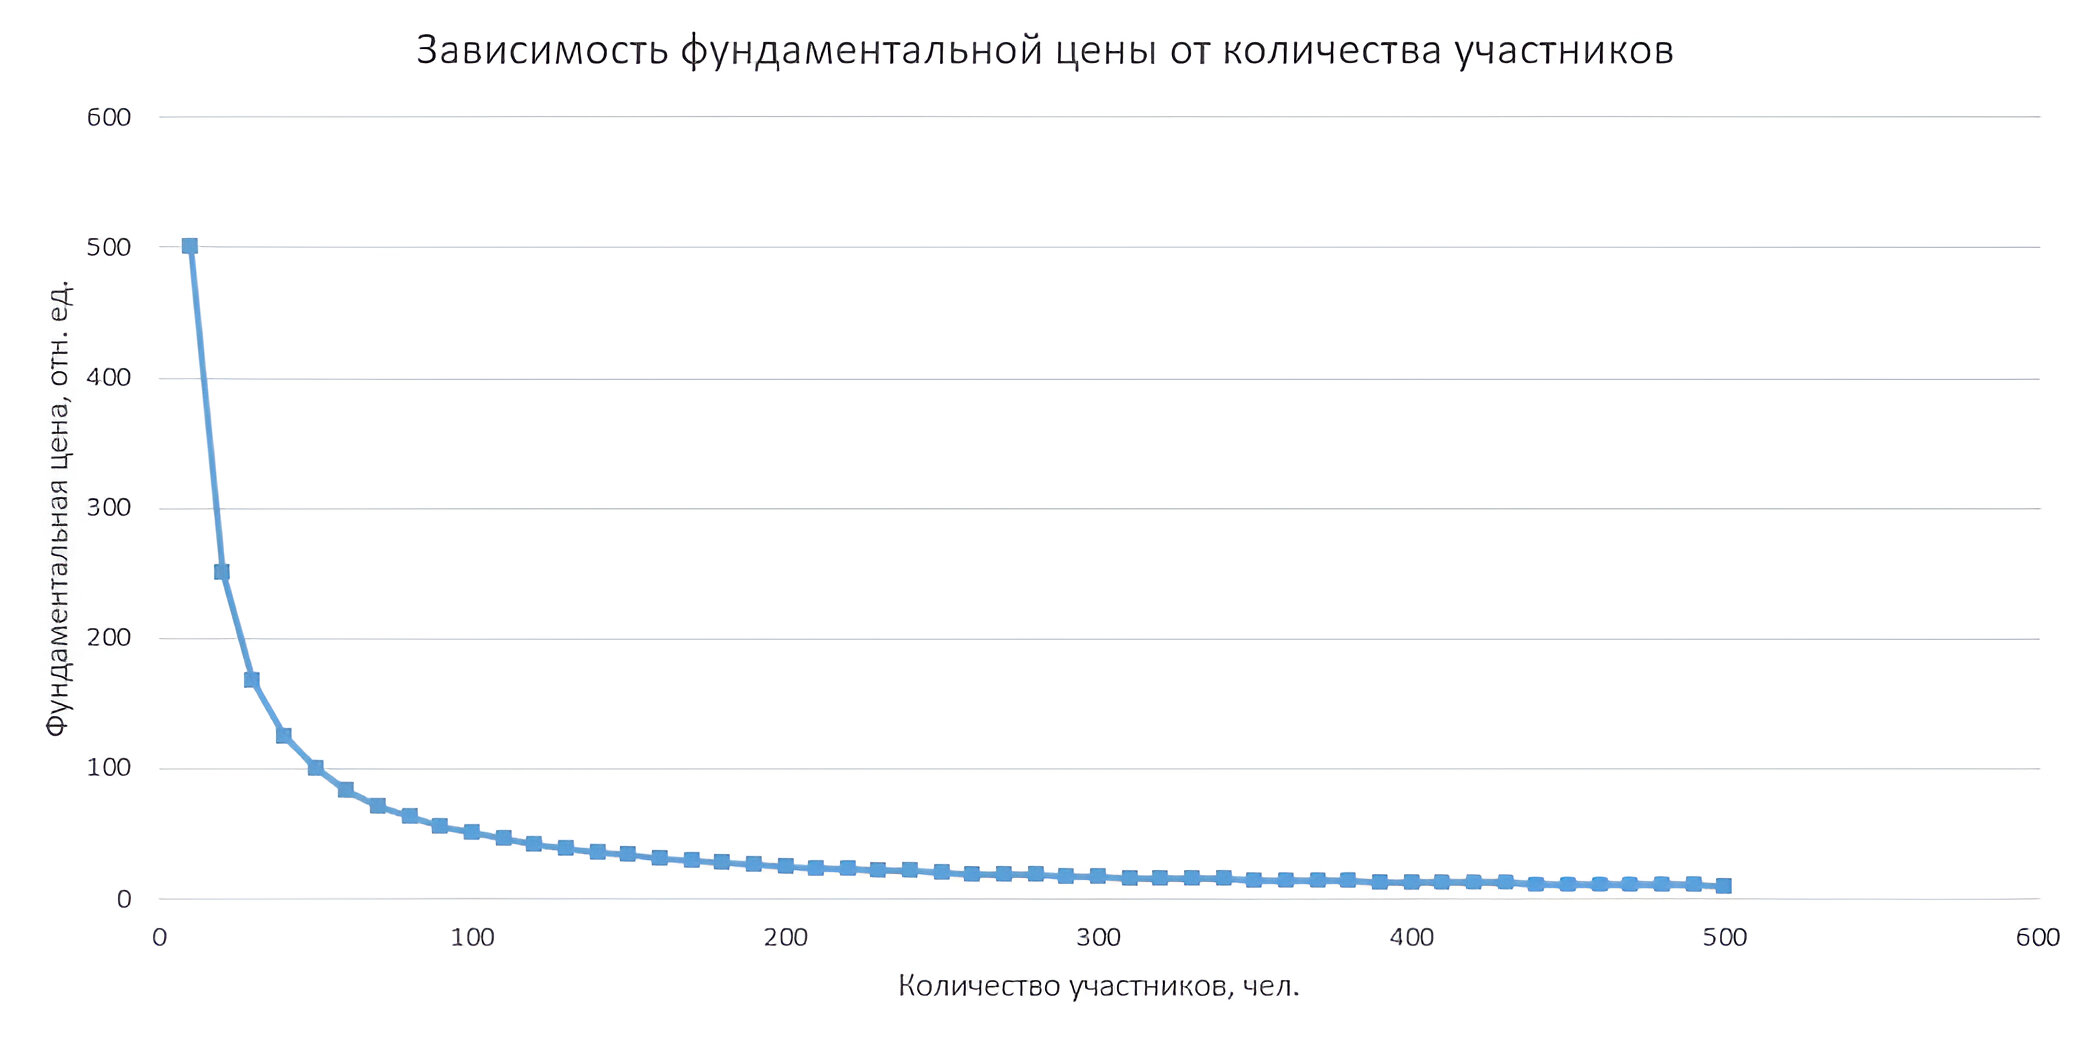
\includegraphics[width=1\textwidth]{images/dependency-1.png}
	\caption{График зависимости значения фундаментальной цены от количества участников} 
	\label{fig:dependency-1} 
\end{figure}

\section{Определение зависимости значения фундаментальной цены от стоимости мероприятия}

Для определения зависимости используется мероприятие, состоящее из 3-х дней с одинаковым количеством участников равным 500.

Результаты определения зависимости значения фундаментальной цены от стоимости мероприятия представлены в таблицах~\ref{tbl:short-dependence-2}~и~\ref{tbl:dependence-2}.

\begin{table}[H]
	\centering
	\caption{Результаты определения зависимости значения фундаментальной цены от стоимости мероприятия}
	\label{tbl:short-dependence-2}
	\begin{tabularx}{\textwidth}{|X|X|}
		\hline
		\textbf{Стоимость мероприятия} & \textbf{Фундаментальная цена} \\
		\hline
		30 500 & 10 \\ \hline
		33 000 & 15 \\ \hline
		35 500 & 20 \\ \hline
		38 000 & 25 \\ \hline
		40 500 & 30 \\ \hline
		43 000 & 35 \\ \hline
		45 500 & 40 \\ \hline
		48 000 & 45 \\ \hline
		50 500 & 50 \\ \hline
		53 000 & 55 \\ \hline
		55 500 & 60 \\ \hline
	\end{tabularx}
\end{table}

По таблице~\ref{tbl:dependence-2} был построен график~\ref{fig:dependency-2}, который наглядно демонстрирует результаты определения зависимости значения фундаментальной цены от стоимости мероприятия. Исходя из графика можно сделать вывод, что данная зависимость близка к линейной.

\begin{figure}[H]
	\centering
	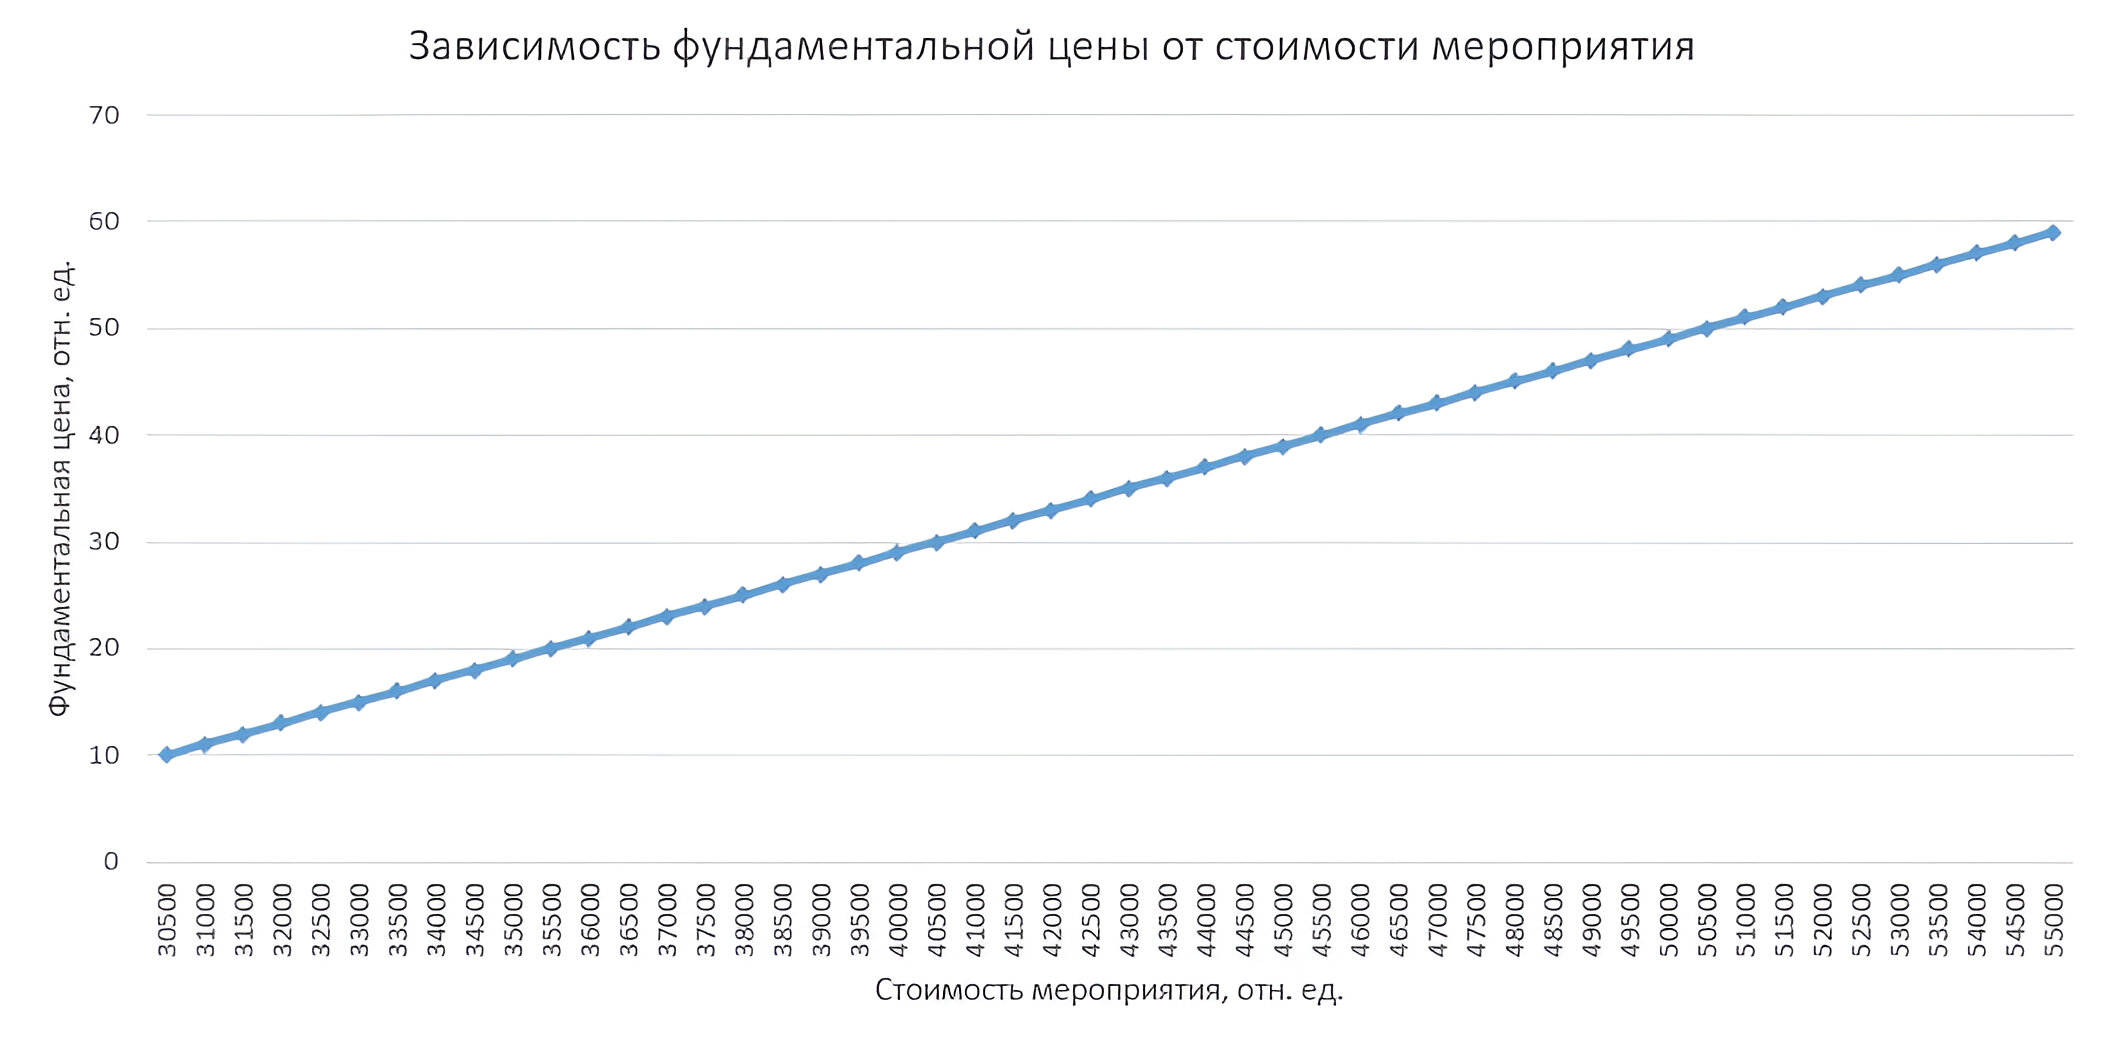
\includegraphics[width=1\textwidth]{images/dependency-2.png}
	\caption{График зависимости значения фундаментальной цены от стоимости мероприятия} 
	\label{fig:dependency-2} 
\end{figure}

\section{Вывод}

В этой части были представлены технические характеристики, постановка, проведение и результаты исследования.

\clearpage
